\beginsong{Und wir kauern wieder um die heiße Glut}[wuw={Fredl Mayr}, pfii={18}, pfiii={63}, bo={332}, index={Und wir kauern wieder}]

\markboth{\songtitle}{\songtitle}

\beginverse
\endverse

\centering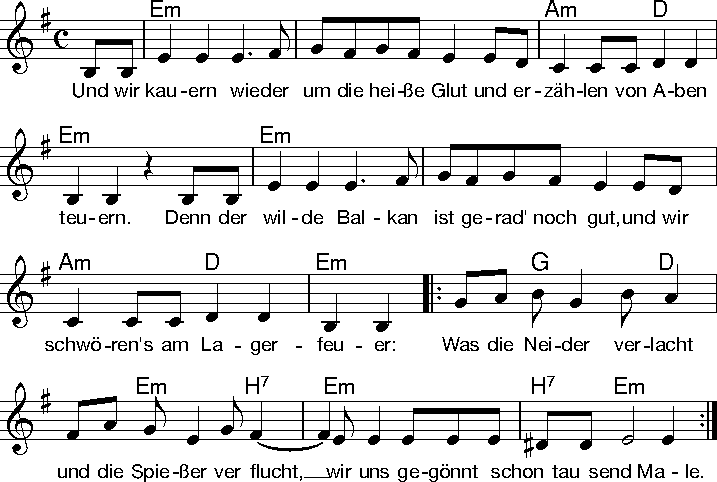
\includegraphics[width=1\textwidth]{Noten/Lied088.pdf}	

\beginverse
Doch sehr \[Em]bald wird es wahr, dass wir stehen am Meer 
und ge\[Am]denken der \[D]fernen \[Em]Heimat, 
denn der kleine Trupp, er rüstet sich sehr, 
zu ver\[Am]lassen die \[D]grauen \[Em]Mauern. 
\lrep Und es \[G]fällt uns nicht \[D]schwer und wir \[Em]freuen uns \[H7]sehr, 
\[Em]bald flattern Se\[H7]gel 'gen \[Em]Osten. \rrep
\endverse

\beginverse
Und der ^Silberfalke flattert uns voran, 
auf der ^weiß-blauen ^Fahne am ^Maste.
Und als wildes Lied schwingt sich von Kahn zu Kahn 
das be^kannte, das ^vielfach ver^hasste, 
\lrep das die ^Neider ver^dammt und die ^Spießer ver^flucht, 
^die uns gehemmt viel^tausend ^Male. \rrep
\endverse

\endsong

\beginscripture{} 

\endscripture

\begin{intersong}
\ifthenelse{\boolean{pics}}{
\ThisLRCornerWallPaper{0.8}{Bilder/undwirkauern2.png}
}{}

\end{intersong}
